

\begin{frame}{\ft{Using Embedded RETS Data}}

\doubleFrame{Each Re-PDF file is a vehicle for 
delivering a pre-selected assembly of RETS 
(Real Estate Transaction Standard) data to 
prospective buyers.  With RETS data selected 
in advance, the Re-PDF application 
can focus on presenting this data 
in the most compelling, interactive ways.}

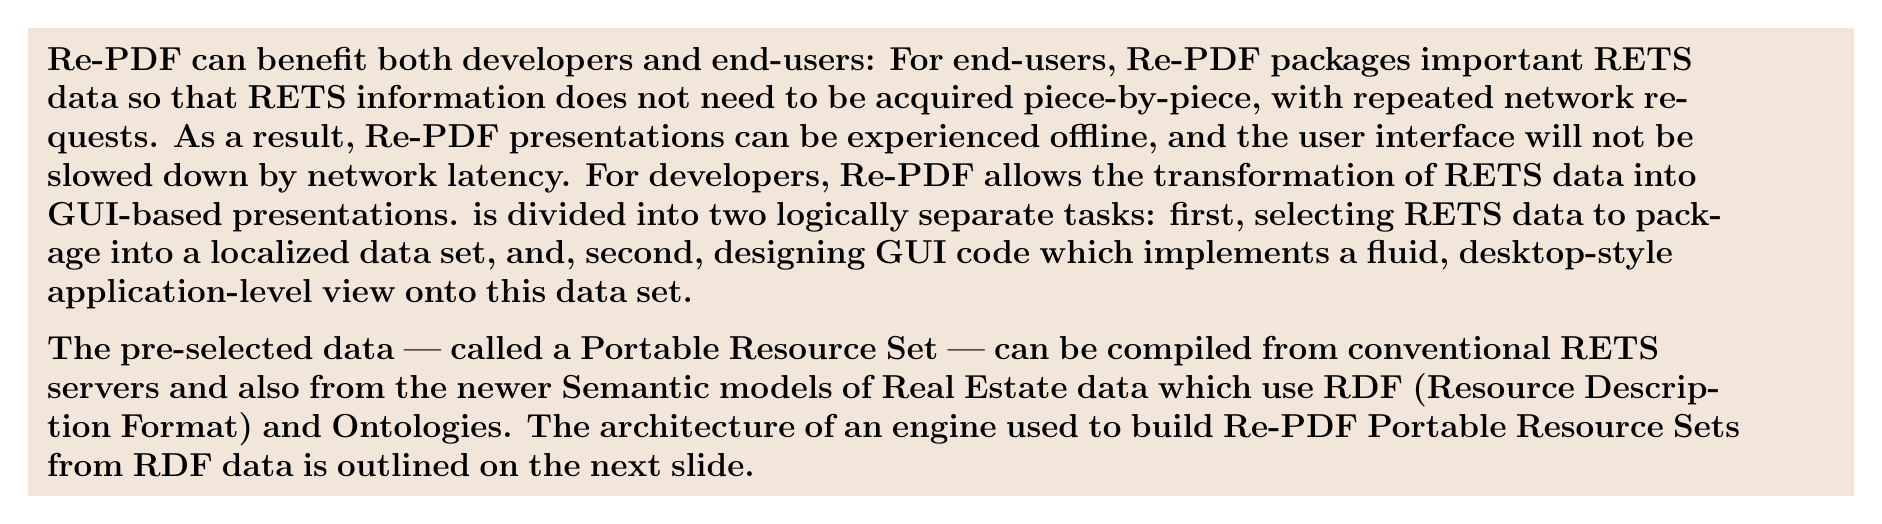
\begin{tikzpicture}
\nodeincludegraphicsTR{6.18cm}{1cm}{screenshots/ss-loaded.png}

 \node [anchor=west,fill=brown!20!white,inner sep=7, text width=22.7cm]
  (longnote) at (0.2,7.8) {%  %{\color{rb!85!red}{
  {\cframedbox{\large 
  {%
  \begin{minipage}{21.9cm}
  {\textbf{Re-PDF can benefit both developers and 
  end-users:  For end-users, Re-PDF packages important 
  RETS data so that RETS information does not need to be 
  acquired piece-by-piece, with repeated network requests.  As 
  a result, Re-PDF presentations can be experienced offline, 
  and the user interface will not be slowed down by network latency.  
  For developers, Re-PDF allows the transformation of RETS 
  data into GUI-based presentations.  
   is divided into 
  two logically separate tasks: first, selecting RETS data to 
  package into a localized data set, and, second, designing GUI 
  code which implements a fluid, desktop-style application-level 
  view onto this data set.
  \vspace*{0.5em}
  \\
  The pre-selected data --- called 
  a \curlyquote{Portable Resource Set} --- can be compiled from 
  conventional RETS servers and also from the newer 
  \curlyquote{Semantic} models of Real Estate data which use 
  RDF (Resource Description Format) and 
  \curlyquote{Ontologies}.  The architecture of 
  an engine used to build Re-PDF Portable Resource Sets 
  from RDF data is outlined on the next slide.}} 
  
  %{\color{blGreen!40!blbl}Figure \ref{fig:relae}}, 
  %appearing on the next slide.}}
  %
  
  \end{minipage}
  }
  }}};


\end{tikzpicture}


\end{frame}

